The application includes a toggle for visualising the modules within each
microservice. This feature is the visual counterpart to the Modules Comparison
functionality discussed in \Cref{sub:frontend_comparison_microservice_focus}.
However, there is a significant distinction. The toggle for visualising modules
enables users to observe the connections and relationships between modules
across different microservices and microservices from different decompositions.
This capability aids users in visualising the mapping of components from their
original monolithic structure to their placement within microservices.
\Cref{fig:modules_visualisation} illustrates this functionality, showcasing the
visualisation of module connections across microservices, facilitating a
clearer understanding of the distribution and organisation of components within
the application.

\begin{figure*}[!htb]
  \caption{Modules Visualisation} \label{fig:modules_visualisation}
  \centering
  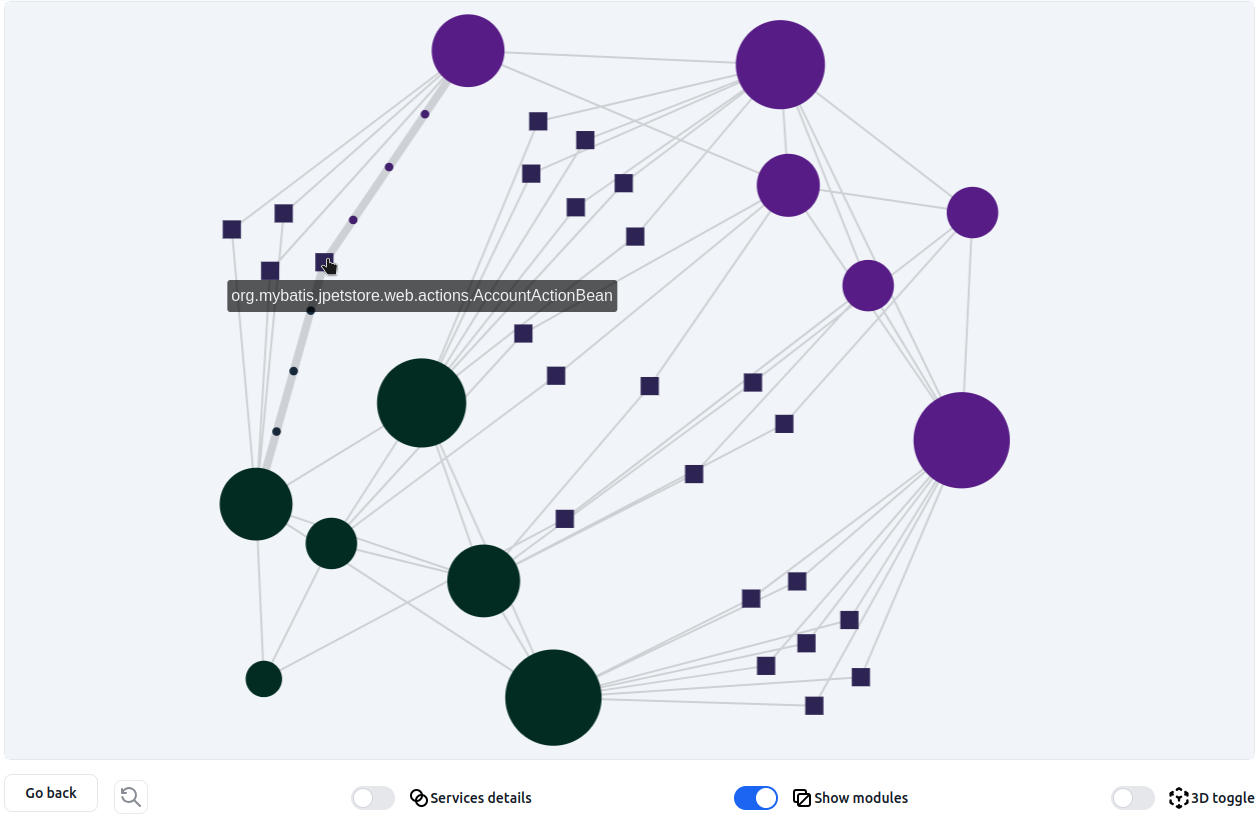
\includegraphics[width=\textwidth]{modules_details}
\end{figure*}
